\chapter{Reward System
	\label{ch:Reward System}}

The \textbf{Reward System} is the last step of Whistle-Blower Application that would be implemented in \textbf {Ethereum Crypto-Currency}.\newline
Reward System is Used for Whistle-Blower when he Upload case and after inquiry the case status would be completed then government make a threshold for Reward in Ethereum that would be Transfer to Whistle-Blower Account after case Complete.    
\section{Ethereum}
\textbf {Ethereum} is an open-source, open, blockchain-based disseminated figuring stage and working framework including savvy contract usefulness. It bolsters an adjusted form of Nakamoto accord by means of exchange based state changes. Ether is a token whose blockchain is produced by the Ethereum stage. 
Ethereum Provides a Platform for Developers to make
Decentralized Application.It Facilitate the Exchange of Money, Property and many
more.
\subsection{Ethereum VS Bitcoin}
The structure of the ethereum blockchain is fundamentally the same as bitcoin's, in that it is a mutual record of the whole exchange history. Each hub on the system stores a duplicate of this history. 

The huge distinction with ethereum is that its hubs store the latest condition of each savvy contract, notwithstanding the majority of the ether exchanges. (This is significantly more entangled than depicted, yet the content beneath should enable you to get your feet wet.) 

For each ethereum application, the system needs to monitor the 'state', or the present data of these applications, including every client's parity, all the keen contract code and where it's everything put away. 

Bitcoin utilizes unspent exchange yields to follow who has how much bitcoin. 

While it sounds increasingly unpredictable, the thought is genuinely basic. Each time a bitcoin exchange is made, the system 'breaks' the aggregate sum as though it was paper cash, issuing back bitcoins such that influences the information to act likewise to physical coins or change. 

To make future exchanges, the bitcoin organize must include every one of your bits of progress, which are classed as either 'spent' or 'unspent'. 

Ethereum, then again, utilizes accounts. 

Like financial balance reserves, ether tokens show up in a wallet, and can be ported (as it were) to another record. Assets are in every case some place, yet don't have what you may call a proceeded with relationship.
\begin{figure}[h]
	\centering
	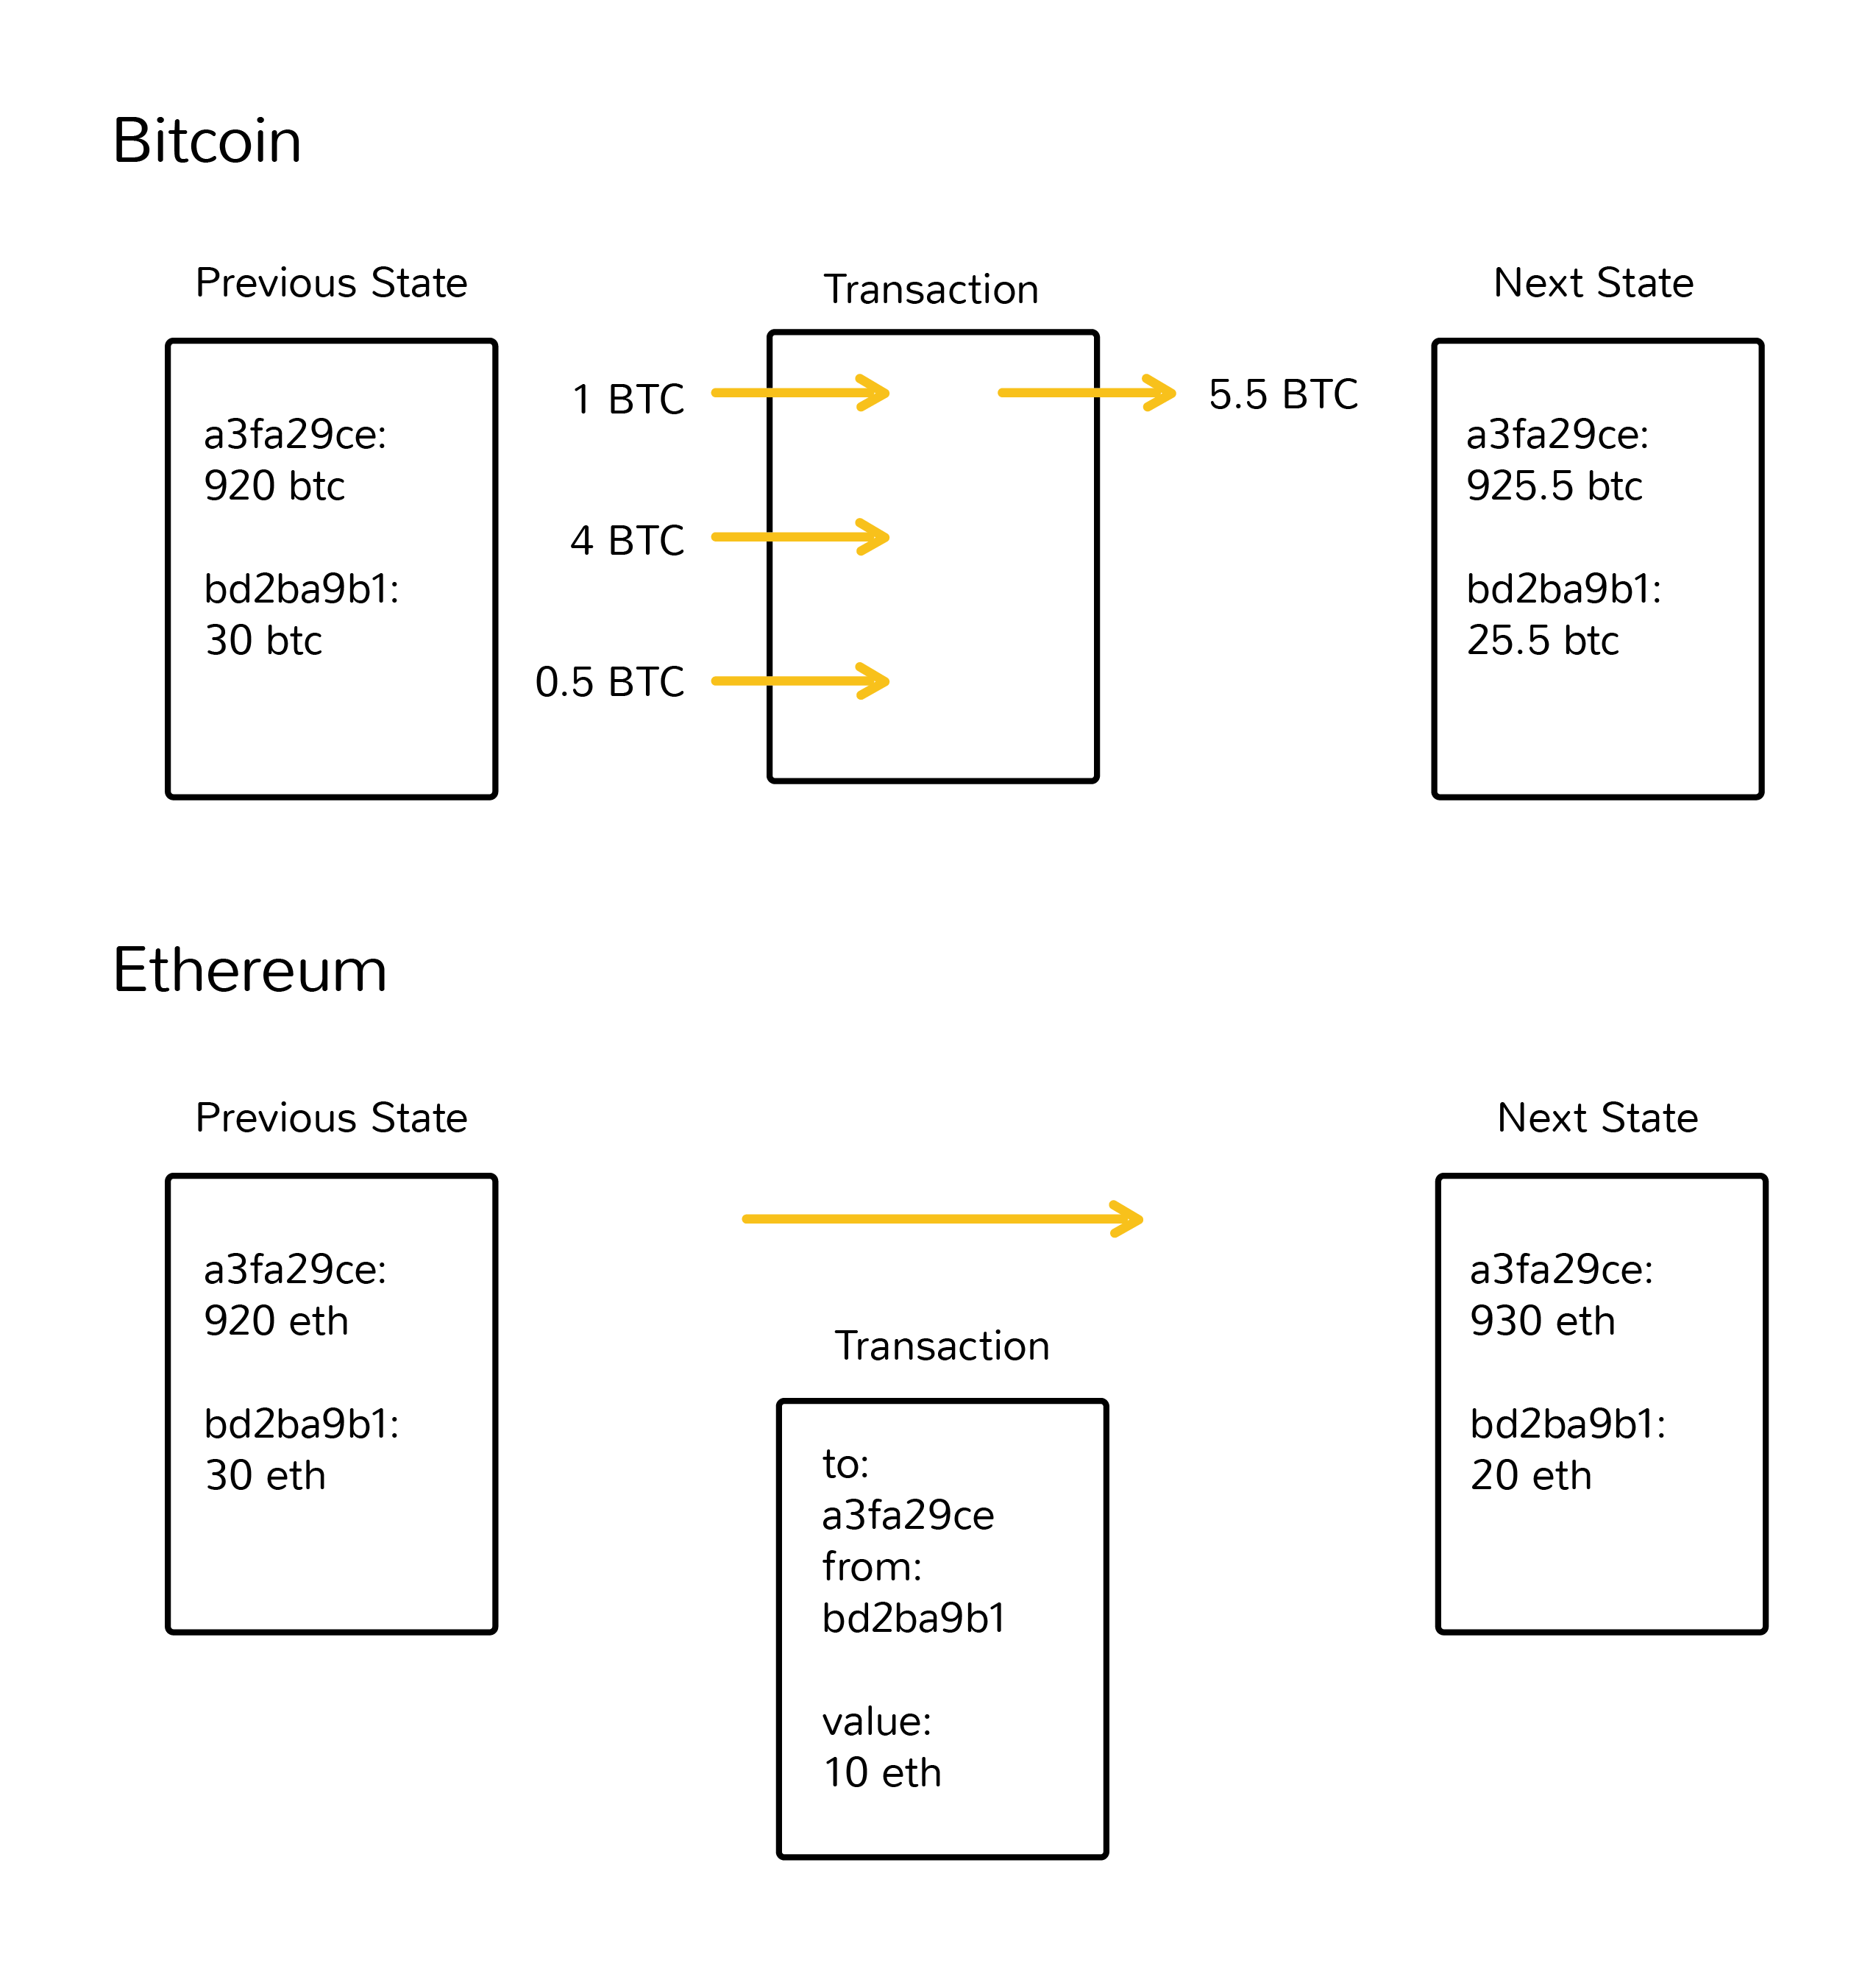
\includegraphics[width=300px]{figures/Ethereum/02.png}
	\caption{Ethereum vs Bitcoin}
	\label{fig:ipfs1}
\end{figure}
\newpage
\subsection{Ethereum Working}
With ethereum, each time a program is utilized, a system of thousands of PCs forms it. 

Contracts written in a brilliant contract-explicit programming dialects are gathered into 'bytecode', which an element called the 'ethereum virtual machine' (EVM) can peruse and execute. 

Every one of the hubs execute this agreement utilizing their EVMs.
\begin{figure}[h]
	\centering
	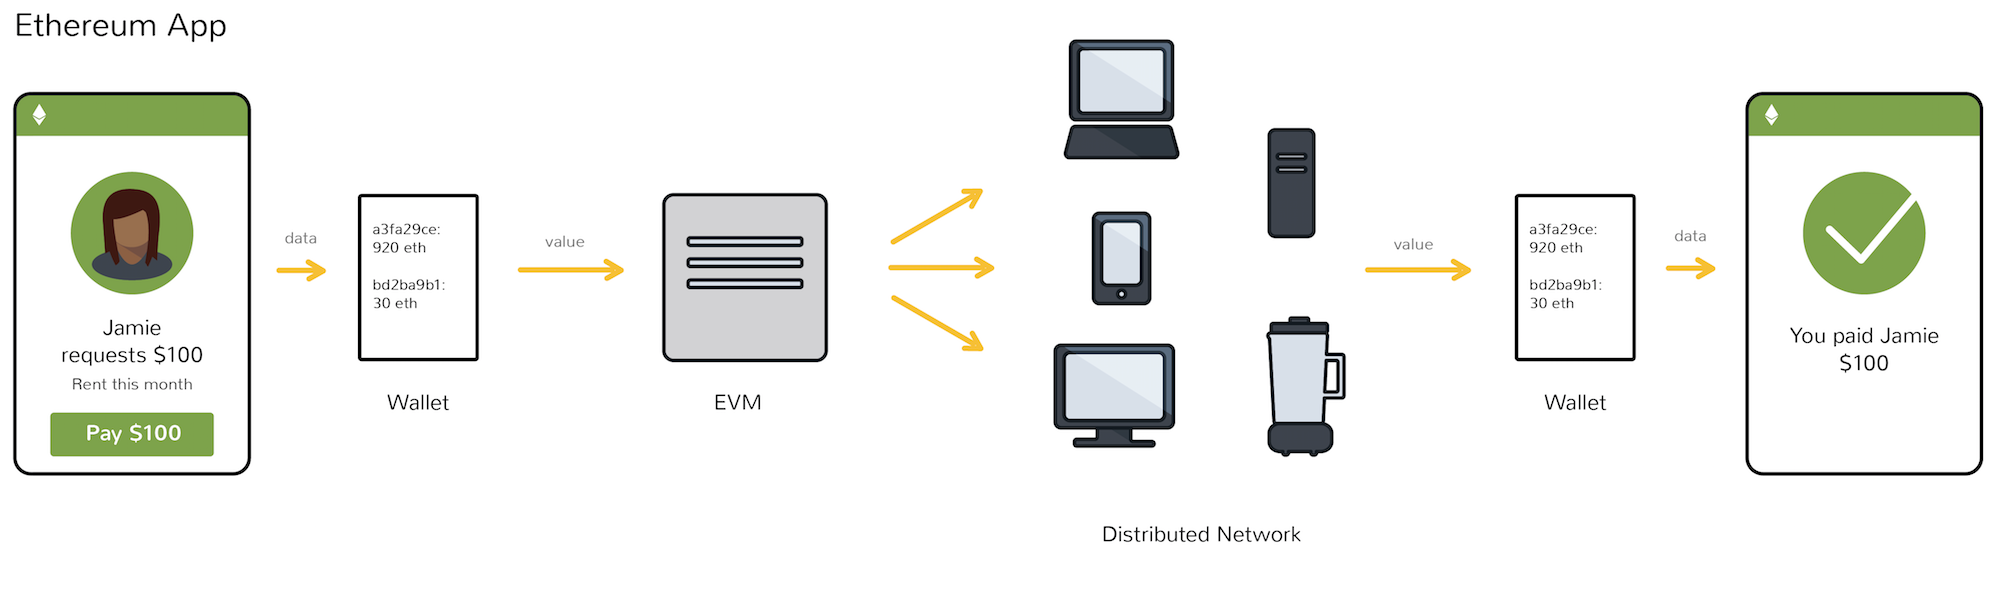
\includegraphics[width=450px]{figures/Ethereum/01.png}
	\caption{Ethereum Working}
	\label{fig:ipfs1}
\end{figure}

Keep in mind that each hub in the system holds a duplicate of the exchange and savvy contract history of the system, notwithstanding monitoring the current 'state'. Each time a client plays out some activity, the majority of the hubs on the system need to come to understanding that this change occurred. 

The objective here is for the system of excavators and hubs to assume liability for exchanging the move from state to state, instead of some expert, for example, PayPal or a bank. Bitcoin excavators approve the move of responsibility for starting with one individual then onto the next. The EVM executes an agreement with whatever administers the engineer at first modified. 

Real calculation on the EVM is accomplished through a stack-based bytecode language (the zeroes that a machine can peruse), however designers can compose keen contracts in abnormal state dialects, for example, Solidity and Serpent that are simpler for people to peruse and compose. 

As clarified in our guide "How Ethereum Mining Works", excavators are the ones that are anticipating awful conduct – like guaranteeing that nobody is spending their cash more than once and dismissing brilliant contracts that haven't been paid for. 

There are a couple of thousand ethereum hubs out there, and each hub is arranging and executing a similar code.


\subsection{Smart Contract In Ethereum}
It's significant that bitcoin was the first to help fundamental shrewd contracts as in the system can exchange an incentive starting with one individual then onto the next. The system of hubs will possibly approve exchanges if certain conditions are met. 
\begin{figure}[h]
	\centering
	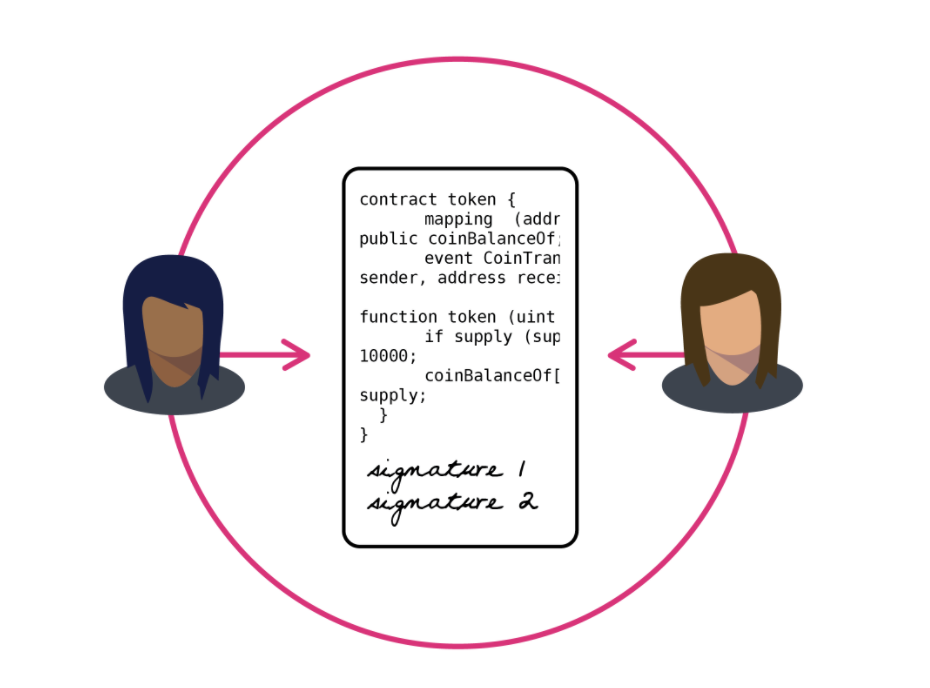
\includegraphics[width=300px]{figures/Ethereum/03.png}
	\caption{Ethereum Smart Contract}
	\label{fig:ipfs1}
\end{figure}
However, bitcoin is constrained to the cash use case. 

On the other hand, ethereum replaces bitcoin's increasingly prohibitive language (a scripting language of a hundred or so contents) and replaces it with a language that enables engineers to compose their very own projects. 

Ethereum enables engineers to program their very own savvy contracts, or 'self-ruling specialists', as the ethereum white paper calls them. The language is 'Turing-finished', which means it bolsters a more extensive arrangement of computational directions.

Shrewd contracts can: 
\begin{itemize}
	\item Capacity as 'multi-signature' accounts, with the goal that reserves are spent just when a required level of individuals concur 
	\item Oversee understandings between clients, state, on the off chance that one purchases protection from the other
	\item Give utility to different contracts (like how a product library works) 
	
	\item Store data around an application, for example, area enlistment data or participation records.
\end{itemize}

\newpage
\section{Ethereum Installation and Integration}
\subsection{Background}
First we should know how our project will interact with the ethereum blockchain. To demonstrate that lets have a look at the picture below.
\begin{figure}[h]
	\centering
	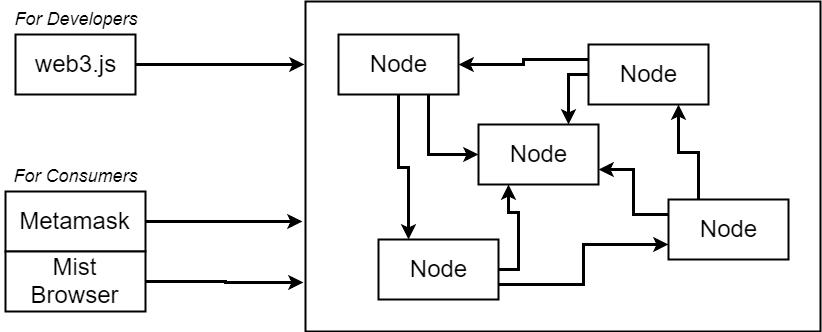
\includegraphics[width=300px]{figures/Ethereum/04.png}
	\caption{Broader View of Ethereum}
	\label{fig:eth4}
\end{figure}

\subsection{Metamask Wallet}
The right block of the diagram shows ethereum nodes and left blocks shows how we can interact with the ethereum network/nodes.Developers uses web3.js library to interact with this ethereum network. Customers/consumers uses Metamask, a browser extention or Mist browser to play with contracts written in ethereum.\\
Metamask provides an ethereum wallet which consists of an account address, public key and a private key. Which can be used for all the four networks provided by ethereum. \textbf{Main} network is ethereum real network and rest of three are for testing purposes.
\begin{figure}[h]
	\centering
	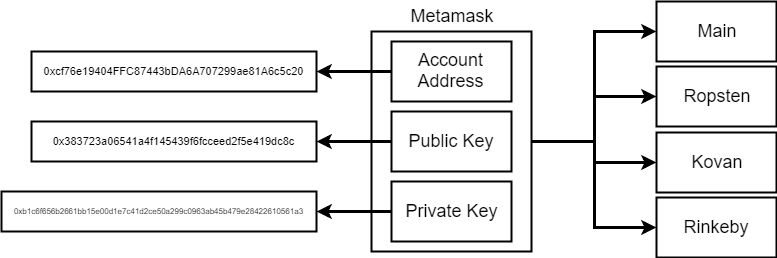
\includegraphics[width=300px]{figures/Ethereum/05.png}
	\caption{Metamask Wallet Structure}
	\label{fig:eth5}
\end{figure}

\subsection{Transaction Structure}
Following bewlow picture demonstrates parameters of a transaction that are required to do a transaction in any ethereum network.
\begin{figure}[h]
	\centering
	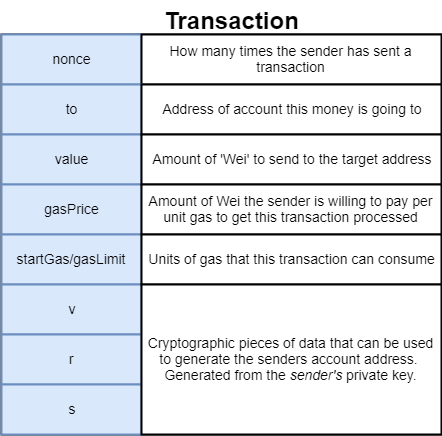
\includegraphics[width=300px]{figures/Ethereum/06.png}
	\caption{Ethereum Transaction Structure}
	\label{fig:eth6}
\end{figure}

\subsection{Installation}
Writing contracts in ethereum needs following things.
\begin{itemize}
	\item  Solidity Compiler
	\item  Local or Test Network (Ganache)
\end{itemize}

For writing Contracts in ethereum we'll be using solidity programming language. To compile its code we use solidity compiler. For testing our contracts before deploying our contract to main network we'll be using \textbf{Ganache}.
\newpage 
First we need to create a folder and install the following tools.
\begin{itemize}
	\item  run command " npm init "
	\item  Install solidity compiler by running command " npm install --save solc@0.4.17 "
	\item  Installing local network for ethereum by running command  
	" npm install --save mocha ganache-cli "
\end{itemize}
Stucture of your folder should be as figure below. package.jason file will be added by running npm init command.
\begin{figure}[h]
	\centering
	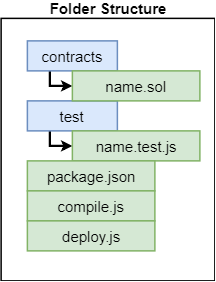
\includegraphics[width=300px]{figures/Ethereum/08.png}
	\caption{Folder Structure}
	\label{fig:eth7}
\end{figure}\newpage

Good to go now you can write your contracts. When contracts are compiled by solidity compiler it gives us its ABI (application binary interface) and contract bytecode. 
\begin{figure}[h]
	\centering
	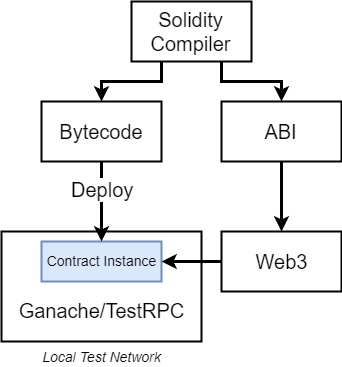
\includegraphics[width=300px]{figures/Ethereum/09.png}
	\caption{Folder Structure}
	\label{fig:eth7}
\end{figure}
\\Our main concern is with the bytecode that is given after compiling by solidity compiler. This bytecode will be used to deploy contracts on our local, test or infact main ethereum network. And ABI will be used by web3.js so that we can interact or write useful fron-ends.